% !TEX encoding = UTF-8 Unicode
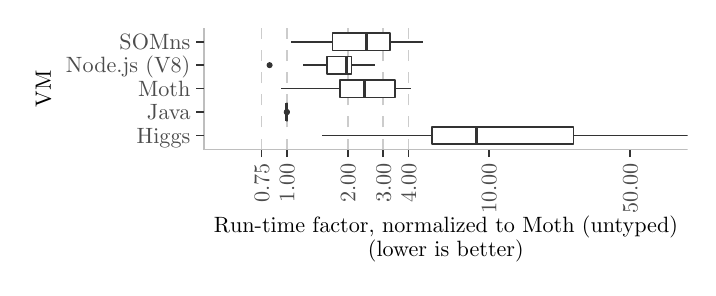
\begin{tikzpicture}[x=1pt,y=1pt]
\definecolor{fillColor}{RGB}{255,255,255}
\path[use as bounding box,fill=fillColor,fill opacity=0.00] (0,0) rectangle (238.49, 86.72);
\begin{scope}
\path[clip] ( 63.73, 42.66) rectangle (238.49, 86.72);
\definecolor{drawColor}{gray}{0.80}

\path[draw=drawColor,line width= 0.6pt,dash pattern=on 4pt off 4pt ,line join=round] ( 84.53, 42.66) -- ( 84.53, 86.72);

\path[draw=drawColor,line width= 0.6pt,dash pattern=on 4pt off 4pt ,line join=round] ( 93.65, 42.66) -- ( 93.65, 86.72);

\path[draw=drawColor,line width= 0.6pt,dash pattern=on 4pt off 4pt ,line join=round] (115.63, 42.66) -- (115.63, 86.72);

\path[draw=drawColor,line width= 0.6pt,dash pattern=on 4pt off 4pt ,line join=round] (128.48, 42.66) -- (128.48, 86.72);

\path[draw=drawColor,line width= 0.6pt,dash pattern=on 4pt off 4pt ,line join=round] (137.61, 42.66) -- (137.61, 86.72);
\definecolor{drawColor}{gray}{0.20}

\path[draw=drawColor,line width= 0.6pt,line join=round] (197.24, 47.75) -- (238.49, 47.75);

\path[draw=drawColor,line width= 0.6pt,line join=round] (146.07, 47.75) -- (106.29, 47.75);
\definecolor{fillColor}{RGB}{255,255,255}

\path[draw=drawColor,line width= 0.6pt,line join=round,line cap=round,fill=fillColor] (197.24, 44.57) --
	(146.07, 44.57) --
	(146.07, 50.92) --
	(197.24, 50.92) --
	(197.24, 44.57) --
	cycle;

\path[draw=drawColor,line width= 1.1pt,line join=round] (162.05, 44.57) -- (162.05, 50.92);
\definecolor{fillColor}{gray}{0.20}

\path[draw=drawColor,line width= 0.4pt,line join=round,line cap=round,fill=fillColor] ( 93.65, 56.22) circle (  0.89);

\path[draw=drawColor,line width= 0.4pt,line join=round,line cap=round,fill=fillColor] ( 93.65, 56.22) circle (  0.89);

\path[draw=drawColor,line width= 0.6pt,line join=round] ( 93.65, 56.22) -- ( 93.65, 56.22);

\path[draw=drawColor,line width= 0.6pt,line join=round] ( 93.65, 56.22) -- ( 93.65, 56.22);
\definecolor{fillColor}{RGB}{255,255,255}

\path[draw=drawColor,line width= 0.6pt,line join=round,line cap=round,fill=fillColor] ( 93.65, 53.04) --
	( 93.65, 53.04) --
	( 93.65, 59.40) --
	( 93.65, 59.40) --
	( 93.65, 53.04) --
	cycle;

\path[draw=drawColor,line width= 1.1pt,line join=round] ( 93.65, 53.04) -- ( 93.65, 59.40);

\path[draw=drawColor,line width= 0.6pt,line join=round] (132.66, 64.69) -- (138.41, 64.69);

\path[draw=drawColor,line width= 0.6pt,line join=round] (112.79, 64.69) -- ( 91.60, 64.69);

\path[draw=drawColor,line width= 0.6pt,line join=round,line cap=round,fill=fillColor] (132.66, 61.52) --
	(112.79, 61.52) --
	(112.79, 67.87) --
	(132.66, 67.87) --
	(132.66, 61.52) --
	cycle;

\path[draw=drawColor,line width= 1.1pt,line join=round] (121.61, 61.52) -- (121.61, 67.87);
\definecolor{fillColor}{gray}{0.20}

\path[draw=drawColor,line width= 0.4pt,line join=round,line cap=round,fill=fillColor] ( 87.41, 73.17) circle (  0.89);

\path[draw=drawColor,line width= 0.6pt,line join=round] (116.97, 73.17) -- (125.64, 73.17);

\path[draw=drawColor,line width= 0.6pt,line join=round] (108.22, 73.17) -- ( 99.51, 73.17);
\definecolor{fillColor}{RGB}{255,255,255}

\path[draw=drawColor,line width= 0.6pt,line join=round,line cap=round,fill=fillColor] (116.97, 69.99) --
	(108.22, 69.99) --
	(108.22, 76.34) --
	(116.97, 76.34) --
	(116.97, 69.99) --
	cycle;

\path[draw=drawColor,line width= 1.1pt,line join=round] (115.22, 69.99) -- (115.22, 76.34);

\path[draw=drawColor,line width= 0.6pt,line join=round] (130.87, 81.64) -- (142.99, 81.64);

\path[draw=drawColor,line width= 0.6pt,line join=round] (110.09, 81.64) -- ( 95.15, 81.64);

\path[draw=drawColor,line width= 0.6pt,line join=round,line cap=round,fill=fillColor] (130.87, 78.46) --
	(110.09, 78.46) --
	(110.09, 84.82) --
	(130.87, 84.82) --
	(130.87, 78.46) --
	cycle;

\path[draw=drawColor,line width= 1.1pt,line join=round] (122.57, 78.46) -- (122.57, 84.82);
\end{scope}
\begin{scope}
\path[clip] (  0.00,  0.00) rectangle (238.49, 86.72);
\definecolor{drawColor}{RGB}{190,190,190}

\path[draw=drawColor,line width= 0.6pt,line join=round] ( 63.73, 42.66) --
	( 63.73, 86.72);
\end{scope}
\begin{scope}
\path[clip] (  0.00,  0.00) rectangle (238.49, 86.72);
\definecolor{drawColor}{gray}{0.30}

\node[text=drawColor,anchor=base east,inner sep=0pt, outer sep=0pt, scale=  0.80] at ( 58.78, 44.99) {Higgs};

\node[text=drawColor,anchor=base east,inner sep=0pt, outer sep=0pt, scale=  0.80] at ( 58.78, 53.46) {Java};

\node[text=drawColor,anchor=base east,inner sep=0pt, outer sep=0pt, scale=  0.80] at ( 58.78, 61.94) {Moth};

\node[text=drawColor,anchor=base east,inner sep=0pt, outer sep=0pt, scale=  0.80] at ( 58.78, 70.41) {Node.js (V8)};

\node[text=drawColor,anchor=base east,inner sep=0pt, outer sep=0pt, scale=  0.80] at ( 58.78, 78.89) {SOMns};
\end{scope}
\begin{scope}
\path[clip] (  0.00,  0.00) rectangle (238.49, 86.72);
\definecolor{drawColor}{gray}{0.20}

\path[draw=drawColor,line width= 0.6pt,line join=round] ( 60.98, 47.75) --
	( 63.73, 47.75);

\path[draw=drawColor,line width= 0.6pt,line join=round] ( 60.98, 56.22) --
	( 63.73, 56.22);

\path[draw=drawColor,line width= 0.6pt,line join=round] ( 60.98, 64.69) --
	( 63.73, 64.69);

\path[draw=drawColor,line width= 0.6pt,line join=round] ( 60.98, 73.17) --
	( 63.73, 73.17);

\path[draw=drawColor,line width= 0.6pt,line join=round] ( 60.98, 81.64) --
	( 63.73, 81.64);
\end{scope}
\begin{scope}
\path[clip] (  0.00,  0.00) rectangle (238.49, 86.72);
\definecolor{drawColor}{RGB}{190,190,190}

\path[draw=drawColor,line width= 0.6pt,line join=round] ( 63.73, 42.66) --
	(238.49, 42.66);
\end{scope}
\begin{scope}
\path[clip] (  0.00,  0.00) rectangle (238.49, 86.72);
\definecolor{drawColor}{gray}{0.20}

\path[draw=drawColor,line width= 0.6pt,line join=round] ( 84.53, 39.91) --
	( 84.53, 42.66);

\path[draw=drawColor,line width= 0.6pt,line join=round] ( 93.65, 39.91) --
	( 93.65, 42.66);

\path[draw=drawColor,line width= 0.6pt,line join=round] (115.63, 39.91) --
	(115.63, 42.66);

\path[draw=drawColor,line width= 0.6pt,line join=round] (128.48, 39.91) --
	(128.48, 42.66);

\path[draw=drawColor,line width= 0.6pt,line join=round] (137.61, 39.91) --
	(137.61, 42.66);

\path[draw=drawColor,line width= 0.6pt,line join=round] (166.66, 39.91) --
	(166.66, 42.66);

\path[draw=drawColor,line width= 0.6pt,line join=round] (217.69, 39.91) --
	(217.69, 42.66);
\end{scope}
\begin{scope}
\path[clip] (  0.00,  0.00) rectangle (238.49, 86.72);
\definecolor{drawColor}{gray}{0.30}

\node[text=drawColor,rotate= 90.00,anchor=base east,inner sep=0pt, outer sep=0pt, scale=  0.80] at ( 87.28, 37.71) {0.75};

\node[text=drawColor,rotate= 90.00,anchor=base east,inner sep=0pt, outer sep=0pt, scale=  0.80] at ( 96.40, 37.71) {1.00};

\node[text=drawColor,rotate= 90.00,anchor=base east,inner sep=0pt, outer sep=0pt, scale=  0.80] at (118.38, 37.71) {2.00};

\node[text=drawColor,rotate= 90.00,anchor=base east,inner sep=0pt, outer sep=0pt, scale=  0.80] at (131.24, 37.71) {3.00};

\node[text=drawColor,rotate= 90.00,anchor=base east,inner sep=0pt, outer sep=0pt, scale=  0.80] at (140.36, 37.71) {4.00};

\node[text=drawColor,rotate= 90.00,anchor=base east,inner sep=0pt, outer sep=0pt, scale=  0.80] at (169.41, 37.71) {10.00};

\node[text=drawColor,rotate= 90.00,anchor=base east,inner sep=0pt, outer sep=0pt, scale=  0.80] at (220.45, 37.71) {50.00};
\end{scope}
\begin{scope}
\path[clip] (  0.00,  0.00) rectangle (238.49, 86.72);
\definecolor{drawColor}{RGB}{0,0,0}

\node[text=drawColor,anchor=base,inner sep=0pt, outer sep=0pt, scale=  0.80] at (151.11, 12.73) {Run-time factor, normalized to Moth (untyped)};

\node[text=drawColor,anchor=base,inner sep=0pt, outer sep=0pt, scale=  0.80] at (151.11,  4.09) {(lower is better)};
\end{scope}
\begin{scope}
\path[clip] (  0.00,  0.00) rectangle (238.49, 86.72);
\definecolor{drawColor}{RGB}{0,0,0}

\node[text=drawColor,rotate= 90.00,anchor=base,inner sep=0pt, outer sep=0pt, scale=  0.80] at (  8.36, 64.69) {VM};
\end{scope}
\end{tikzpicture}
